% vim:set et sw=2 ts=4 tw=72:

To navigate and inspect the merge-tree view of the kernel we created a
web-based tool called \tool. Creating a web-based tool enables users to
use the system without having to install additional software or store a
large database, making it more accessible, more easily maintainable, and
platform independent. \tool uses the following mechanisms to reach our
goals of better navigation and better explanation of the selected
changes.

\begin{itemize}
        \item Filter by searching
        \item View files edited
        \item View modules
        \item Tree viewer
\end{itemize}

\subsection{Searching}

\begin{figure}
        \centering
        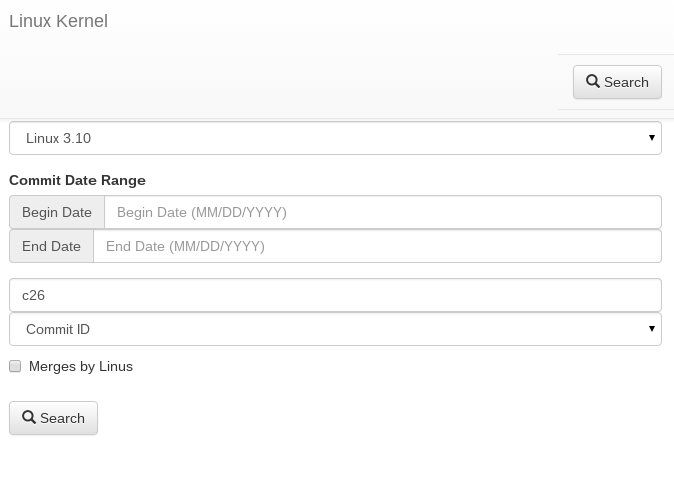
\includegraphics[width=0.47\textwidth]{figures/search.png}
        \caption{Search View allows filtering commits that were merged in a given
                period, filtering by author, keyword, or commit ID.}
        \label{fig:search}
\end{figure}

Searching (depicted in Figure \ref{fig:search}) allows a user to filter
commits and merges that are irrelevant. The search mechanism breaks down
the results by release version. A user can further narrow down the
search by specifying a range of dates in which such commits were merged
by Linus into the master branch---not when the commits were created
(author date and/or commit date). This distinction is important. We have
observed commits that have taken years to arrive into the master
repository after they were originally created.

A user may then provide a search text, filtering by the author name, the
commit ID, or keyword from the log. Any part of the author name may show
up in the results, including searching by email address.

If the user is searching by commit ID, the ID can be specified by using
any of its unique prefixes. For example, the commit
\mycode{3f17ea6dea8ba5668873afa54628a91aaa3fb1c0} is returned when the
user searches for a commit ID of \mycode{3f17e} in the 3.16 Linux
kernel.

\begin{figure}
        \centering
        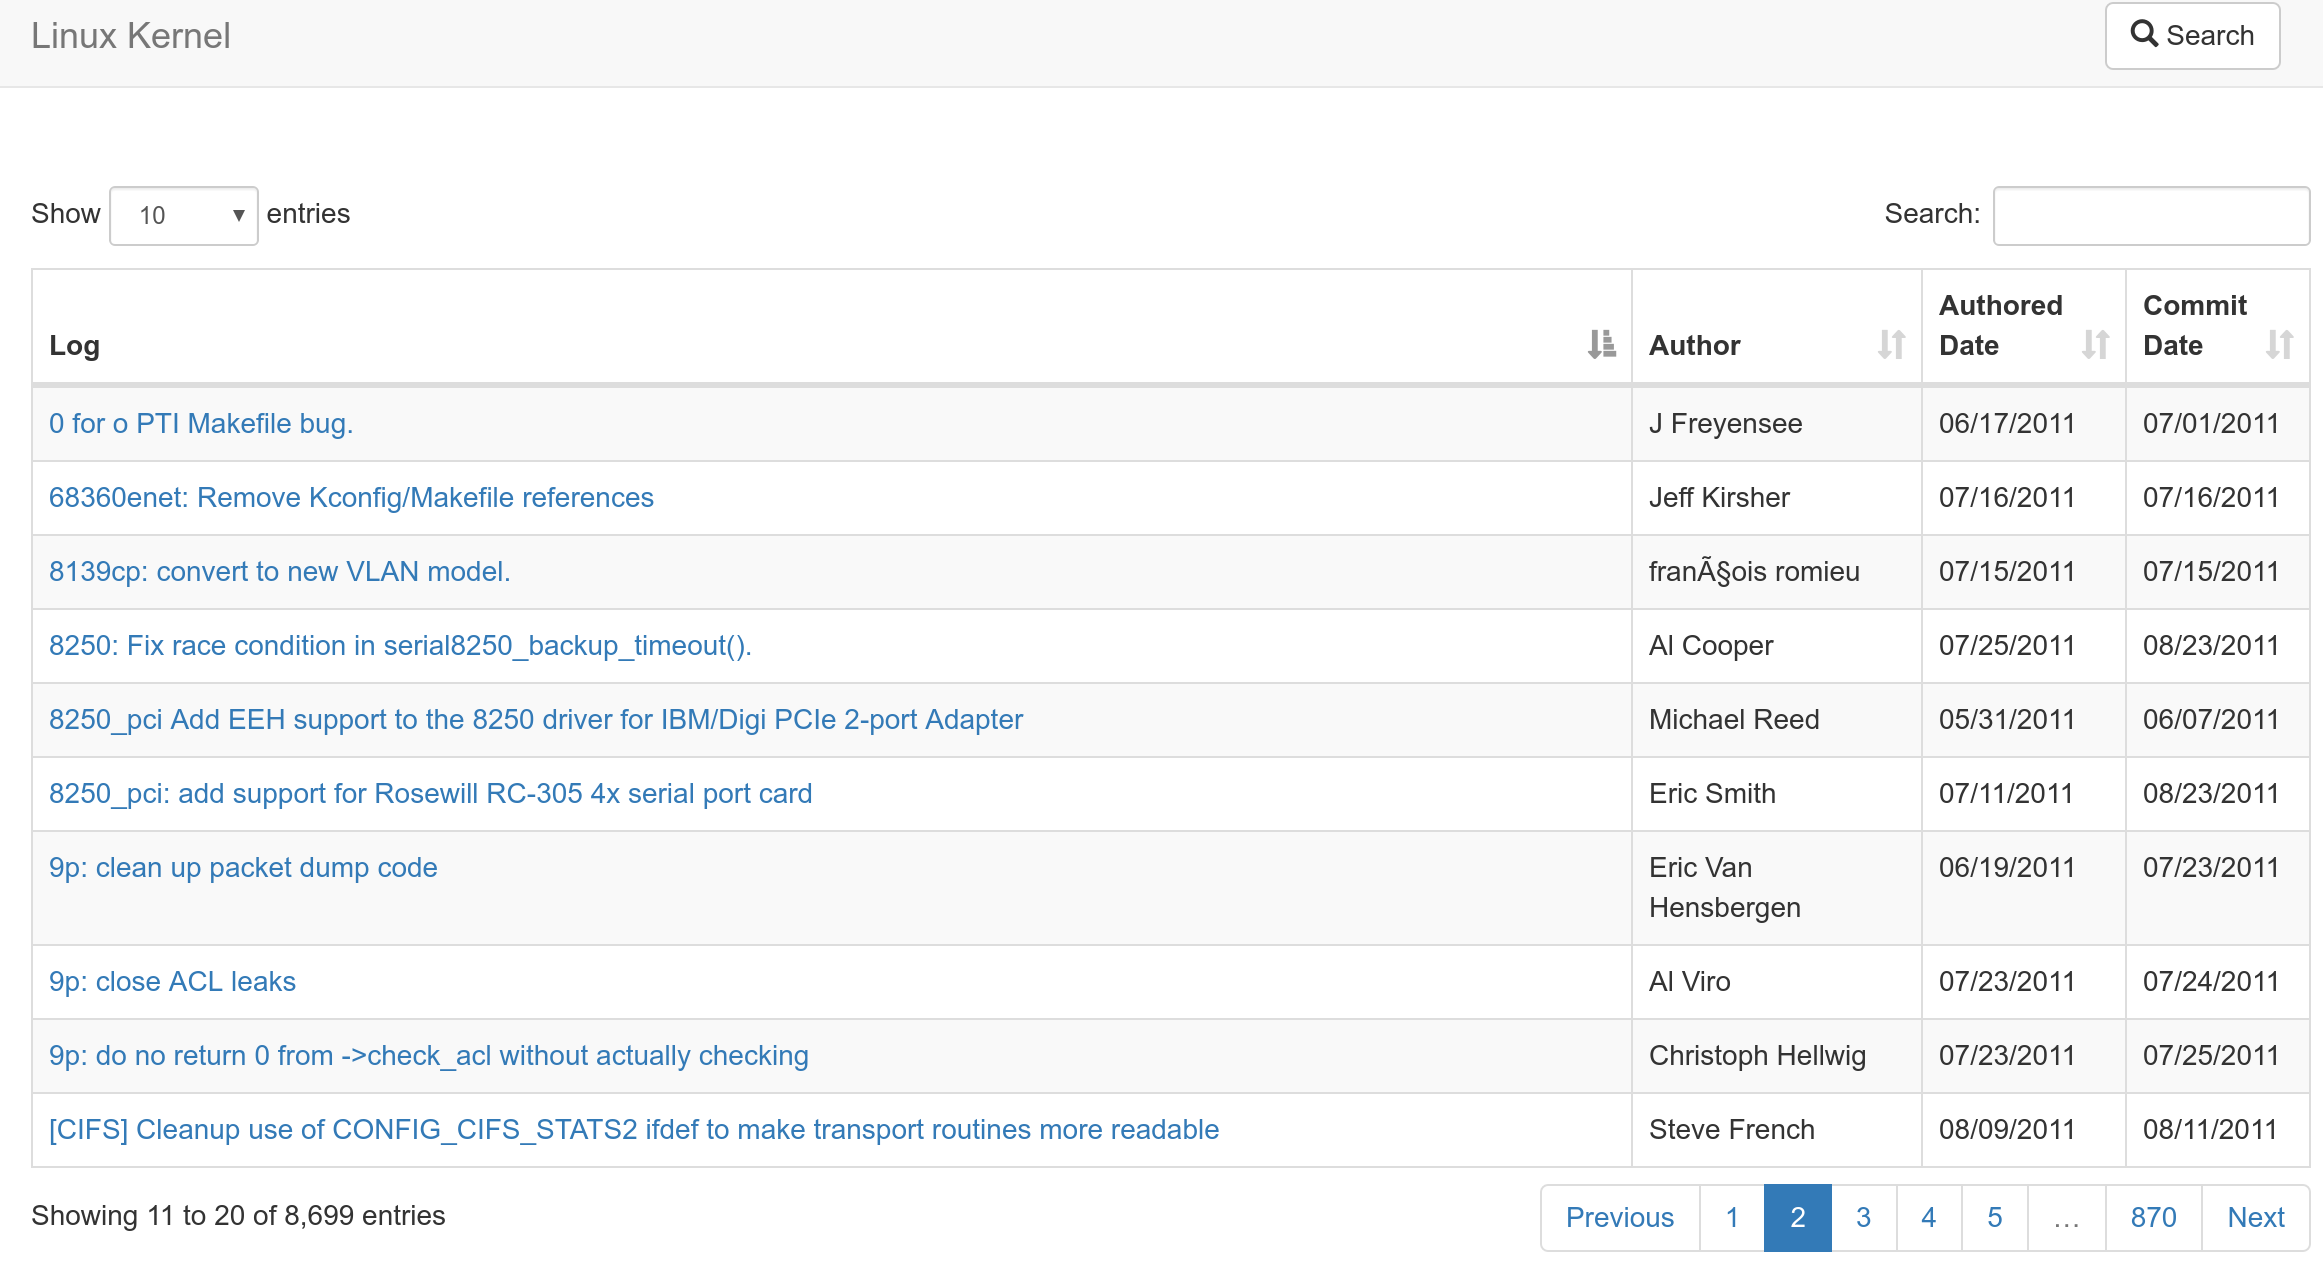
\includegraphics[width=0.47\textwidth]{figures/search_results_2.png}
        \caption{Search Results. Each table entry is a commit merged in the desired
                merged window.}
        \label{fig:results}
\end{figure}

In the search results (seen in Figure~\ref{fig:results}), the user is
presented with the one-line log message preview, the author's name and
email, the date the commit was authored, and the date the commit was
last committed.

\begin{figure}
        \centering
        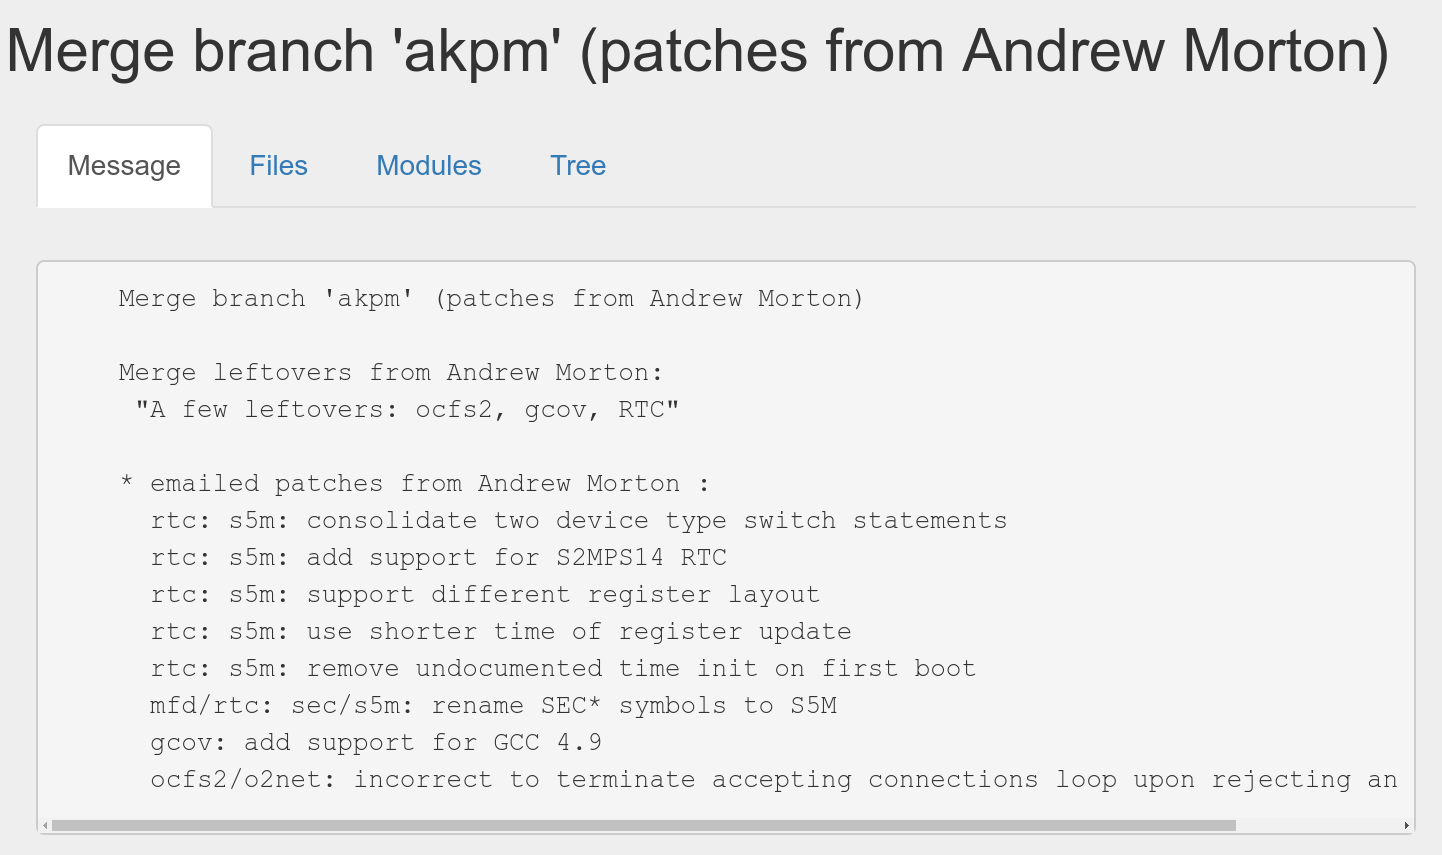
\includegraphics[width=0.47\textwidth]{figures/log_view.png}
        \caption{Panel showing the Commit Message of a commit.}
        \label{fig:message}
\end{figure}

Once a user selects a commit or merge to investigate, they are presented
with a tabbed pane allowing them to view the full commit log, the files
edited, the modules involved, and the merge-tree view.

The first tab displays the full commit log (Figure~\ref{fig:message}).
From this, a user is able to see what they would see had they searched
for the commit using Git log. This doesn't provide additional
information to the other tools, but helps to complete the functionality
of \tool. The commit log provides a user with the information about the
content of the commit and who has signed-off on the commit to ensure
that it is of good quality. The message for merges may contain a summary
of the commits being merged.  The information within these messages is
highly variable, and is completely dependent on the author's style. As
the user moves toward the root-level merge, the quality of these
messages generally improves.

\begin{figure}
        \centering
        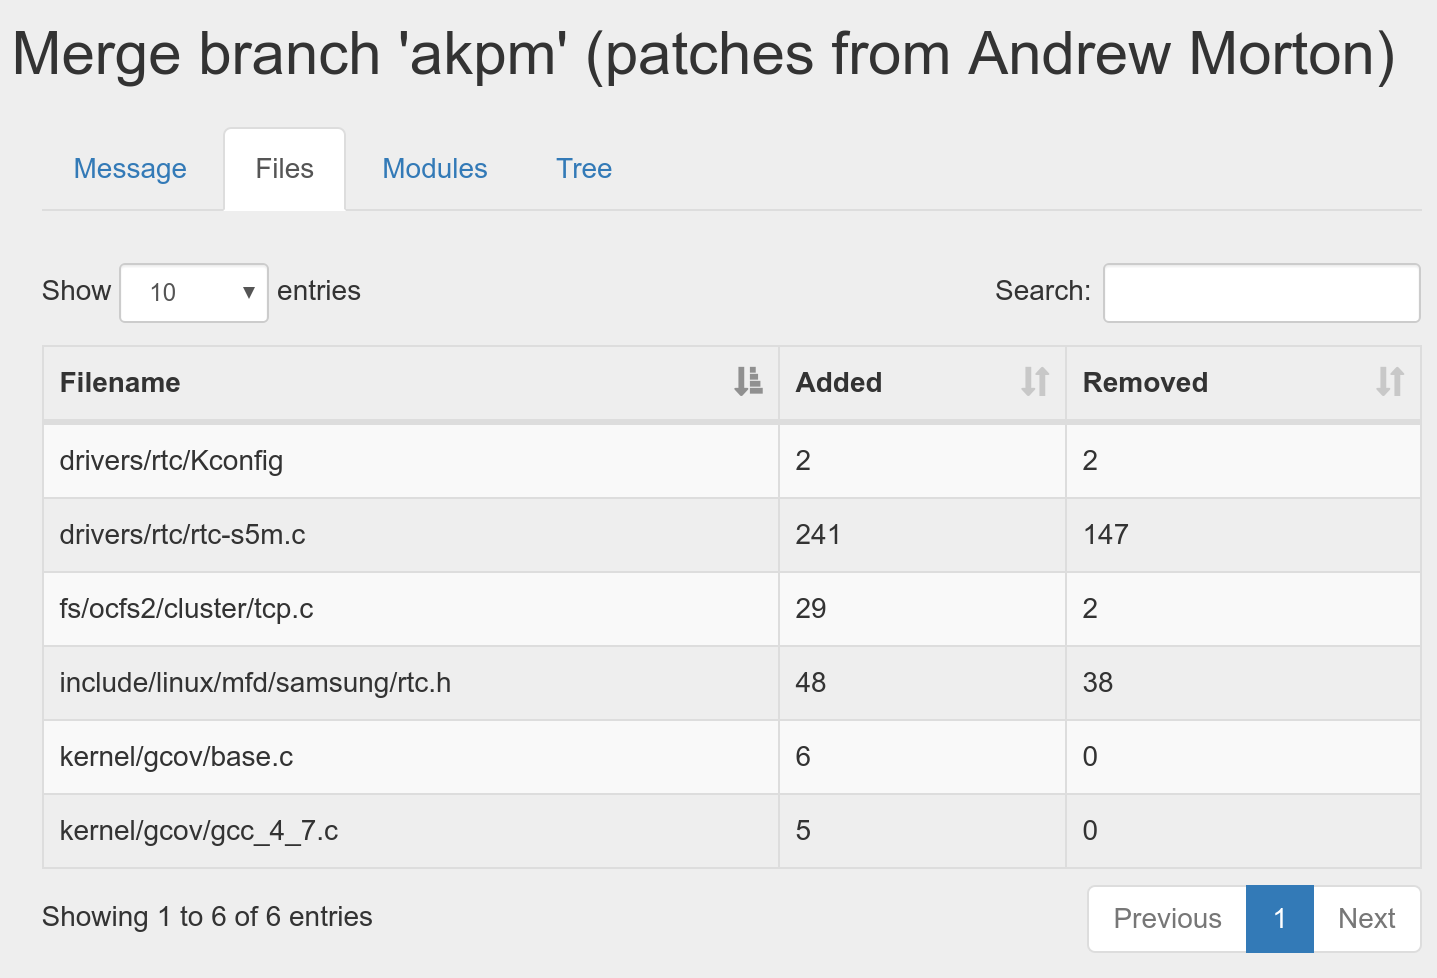
\includegraphics[width=0.47\textwidth]{figures/files_view_2.png}
        \caption{Panel showing the files modified by all the commits that are part
                of this merge.}
        \label{fig:files}
\end{figure}

The second tab is the files tab (Figure~\ref{fig:files}). This tab
provides information on what files have been edited, how many lines were
added, and how many lines were removed in a given commit. For
non-merges, this functionality is similar to the other tools available.
Our tree-based design model allows us to extend this functionality to
merges by aggregating information about all the commits that are
children of the merge in the merge-tree, which other tools are unable to
show. To find the number of lines added to a file in a merge, we take
the sum of the lines added to that file in each of the children of that
merge. We do the same for calculating the number of lines removed.


% This could be extended to use the patch information to determine when a line has been
% replaced rather than incrementing the lines added and removed.

\begin{figure}
        \centering
        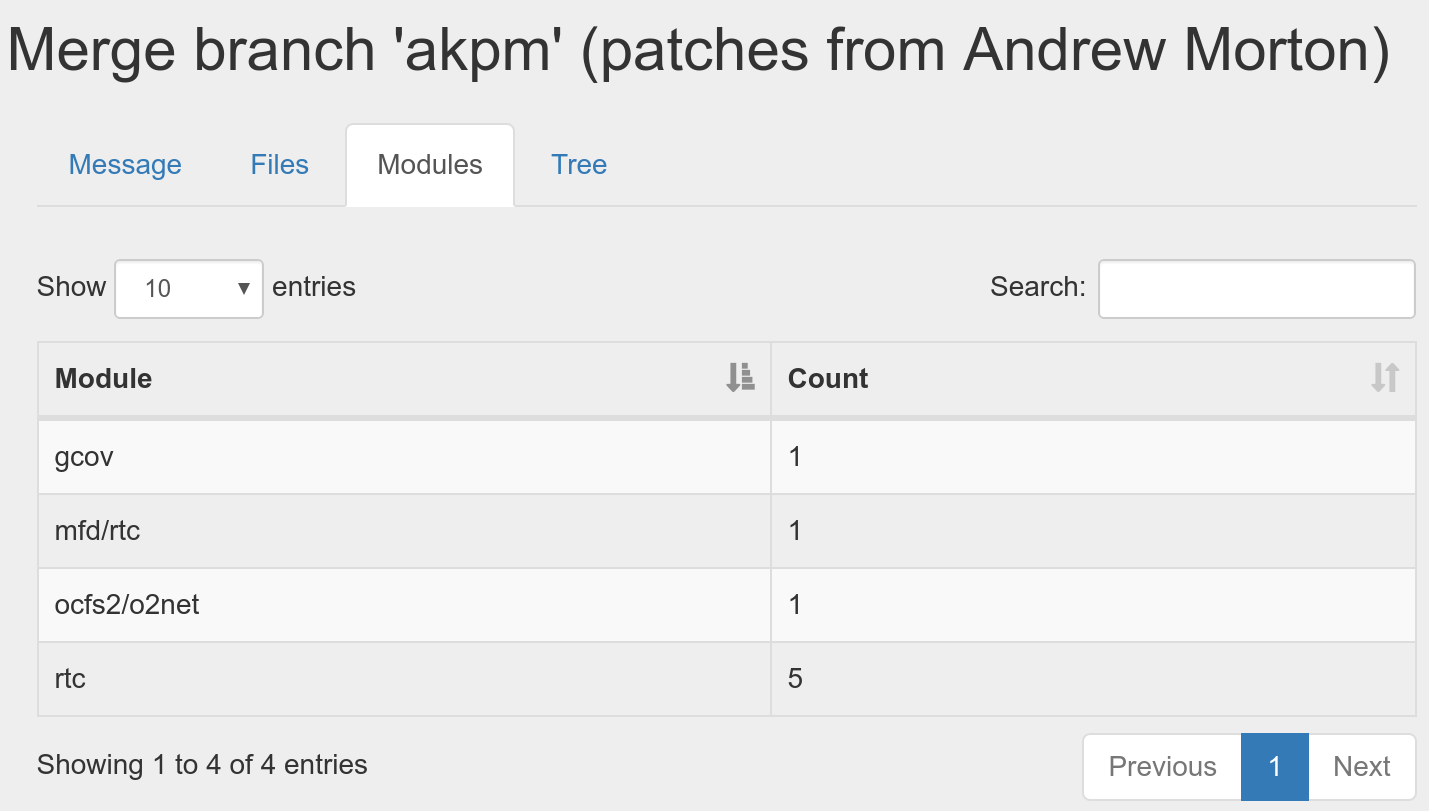
\includegraphics[width=0.47\textwidth]{figures/modules_view_2.png}
        \caption{Panel showing the modules changed by all the commits in this merge.}
        \label{fig:modules}
\end{figure}

The modules tab (Figure~\ref{fig:modules}) shows the modules that are
contained within the commit. Modules are not natively recognized by Git,
and are not going to be present in all repositories. In the Linux
repository, authors put the module they are working on in the one-line
summary of the log-message; for example: the log \emph{gcov: add support
  for FCC 4.9} has updated the \emph{gcov} module (the coverage testing
tool of the kernel). We heuristically extract the module by taking all
text in the log summary of commits until the first colon.  Modules are
logical partitions of the information in the kernel. Depending on where
the author was working, modules can be general, such as ``bluetooth''
and ``wireless'', or can be quite specific for individual hardware, such
as ``ath9k\_hw'' and ``wl1251''. In a few cases, the author of a commit
does not correctly follow this format and the heuristic approach fails.
As with the Files panel, non-merge commits show their corresponding
information, but for merge commits we aggregate all the modules changed
in all the commits that are part of that merge.  The output of this view
is shown in Figure~\ref{fig:modules}.

Finally, we have the Tree view tab. The tree view is designed for
providing easy navigation of the commits within the merge-tree that is
rooted in the current merge.  It also provides a clear topological view
of the merge and the submerges it includes. We have experimented with
various tree designs to find a design that allows for easy navigation
and visualization of both large and small trees. We discuss this panel
in the next subsection.

\subsection{Merge-Tree Views} \label{treeview_section}

The merge-tree view is what makes \tool unique to other tools that
inspect the DAG of a Git repository. With it, a user can inspect how
commits are merged on their way to the master branch. We have
experimented with various types of trees:

\begin{enumerate}
        \item List trees are a text-based representation of the merge-tree, and are easy to search and navigate.
        \item Reingold-Tilford trees provide a clear visual representation of the tree structure of the merge-tree.
        \item Bubble trees organize the data hierarchically by having the parent node contain the child nodes similarly to tree maps, but
                clearly showing the parent-child relationships between commits and merges.
\end{enumerate}


\subsubsection{List Tree}

The list tree viewer (Figure~\ref{fig:list_tree}) is in the form of
nested lists, and is designed to more closely model the tree view found
in file browsers. This tree only contains the commits and merges that
are within the subtrees of the current merge. A commit will never have
any items in this tree as it is a leaf. To accompany the tree, we
include breadcrumbs at the top of the page to enable a user to navigate
both from the root to the leaves and from a leaf to the root. The last
item in the breadcrumb list is the current commit, the previous item is
the parent of the current commit, and the first item is the root merge
into the kernel.

\begin{figure}
        \centering
        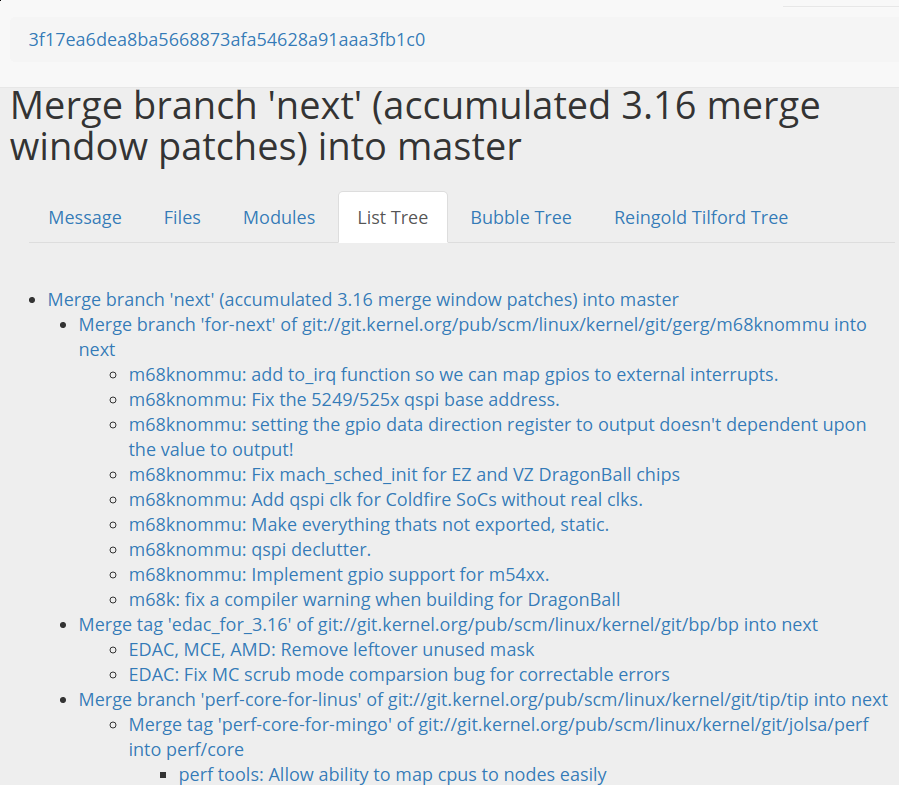
\includegraphics[width=0.47\textwidth]{figures/list_tree.png}
        \caption{List tree view of merge 3f17ea6}
        \label{fig:list_tree}
\end{figure}

\subsubsection{Reingold-Tilford Tree}

The Reingold-Tilford tree\cite{Reingold1981} (Figures
\ref{fig:reingold_tree} and \ref{fig:reingold_tree_zoom}) allows the
visualization and navigation of the entire merge-tree in an intuitive
representation of the tree.  This illustrates a clear notion of root and
leaves, and how to navigate in either direction. Some merge trees are
very large, containing thousands of commits and merged. While the tree
is capable of producing a visualization, it becomes far more difficult
to understand. For example, the merge, 3f17ea6 performed by Linus
Torvalds June 8 2014, contains 7217 commits and merges. \footnote{This
  commit can be inspected at
  \url{http://li.turingmachine/org/commits/3f17ea6dea8ba5668873afa54628a91aaa3fb1c0}}

      \begin{figure}
        \centering
        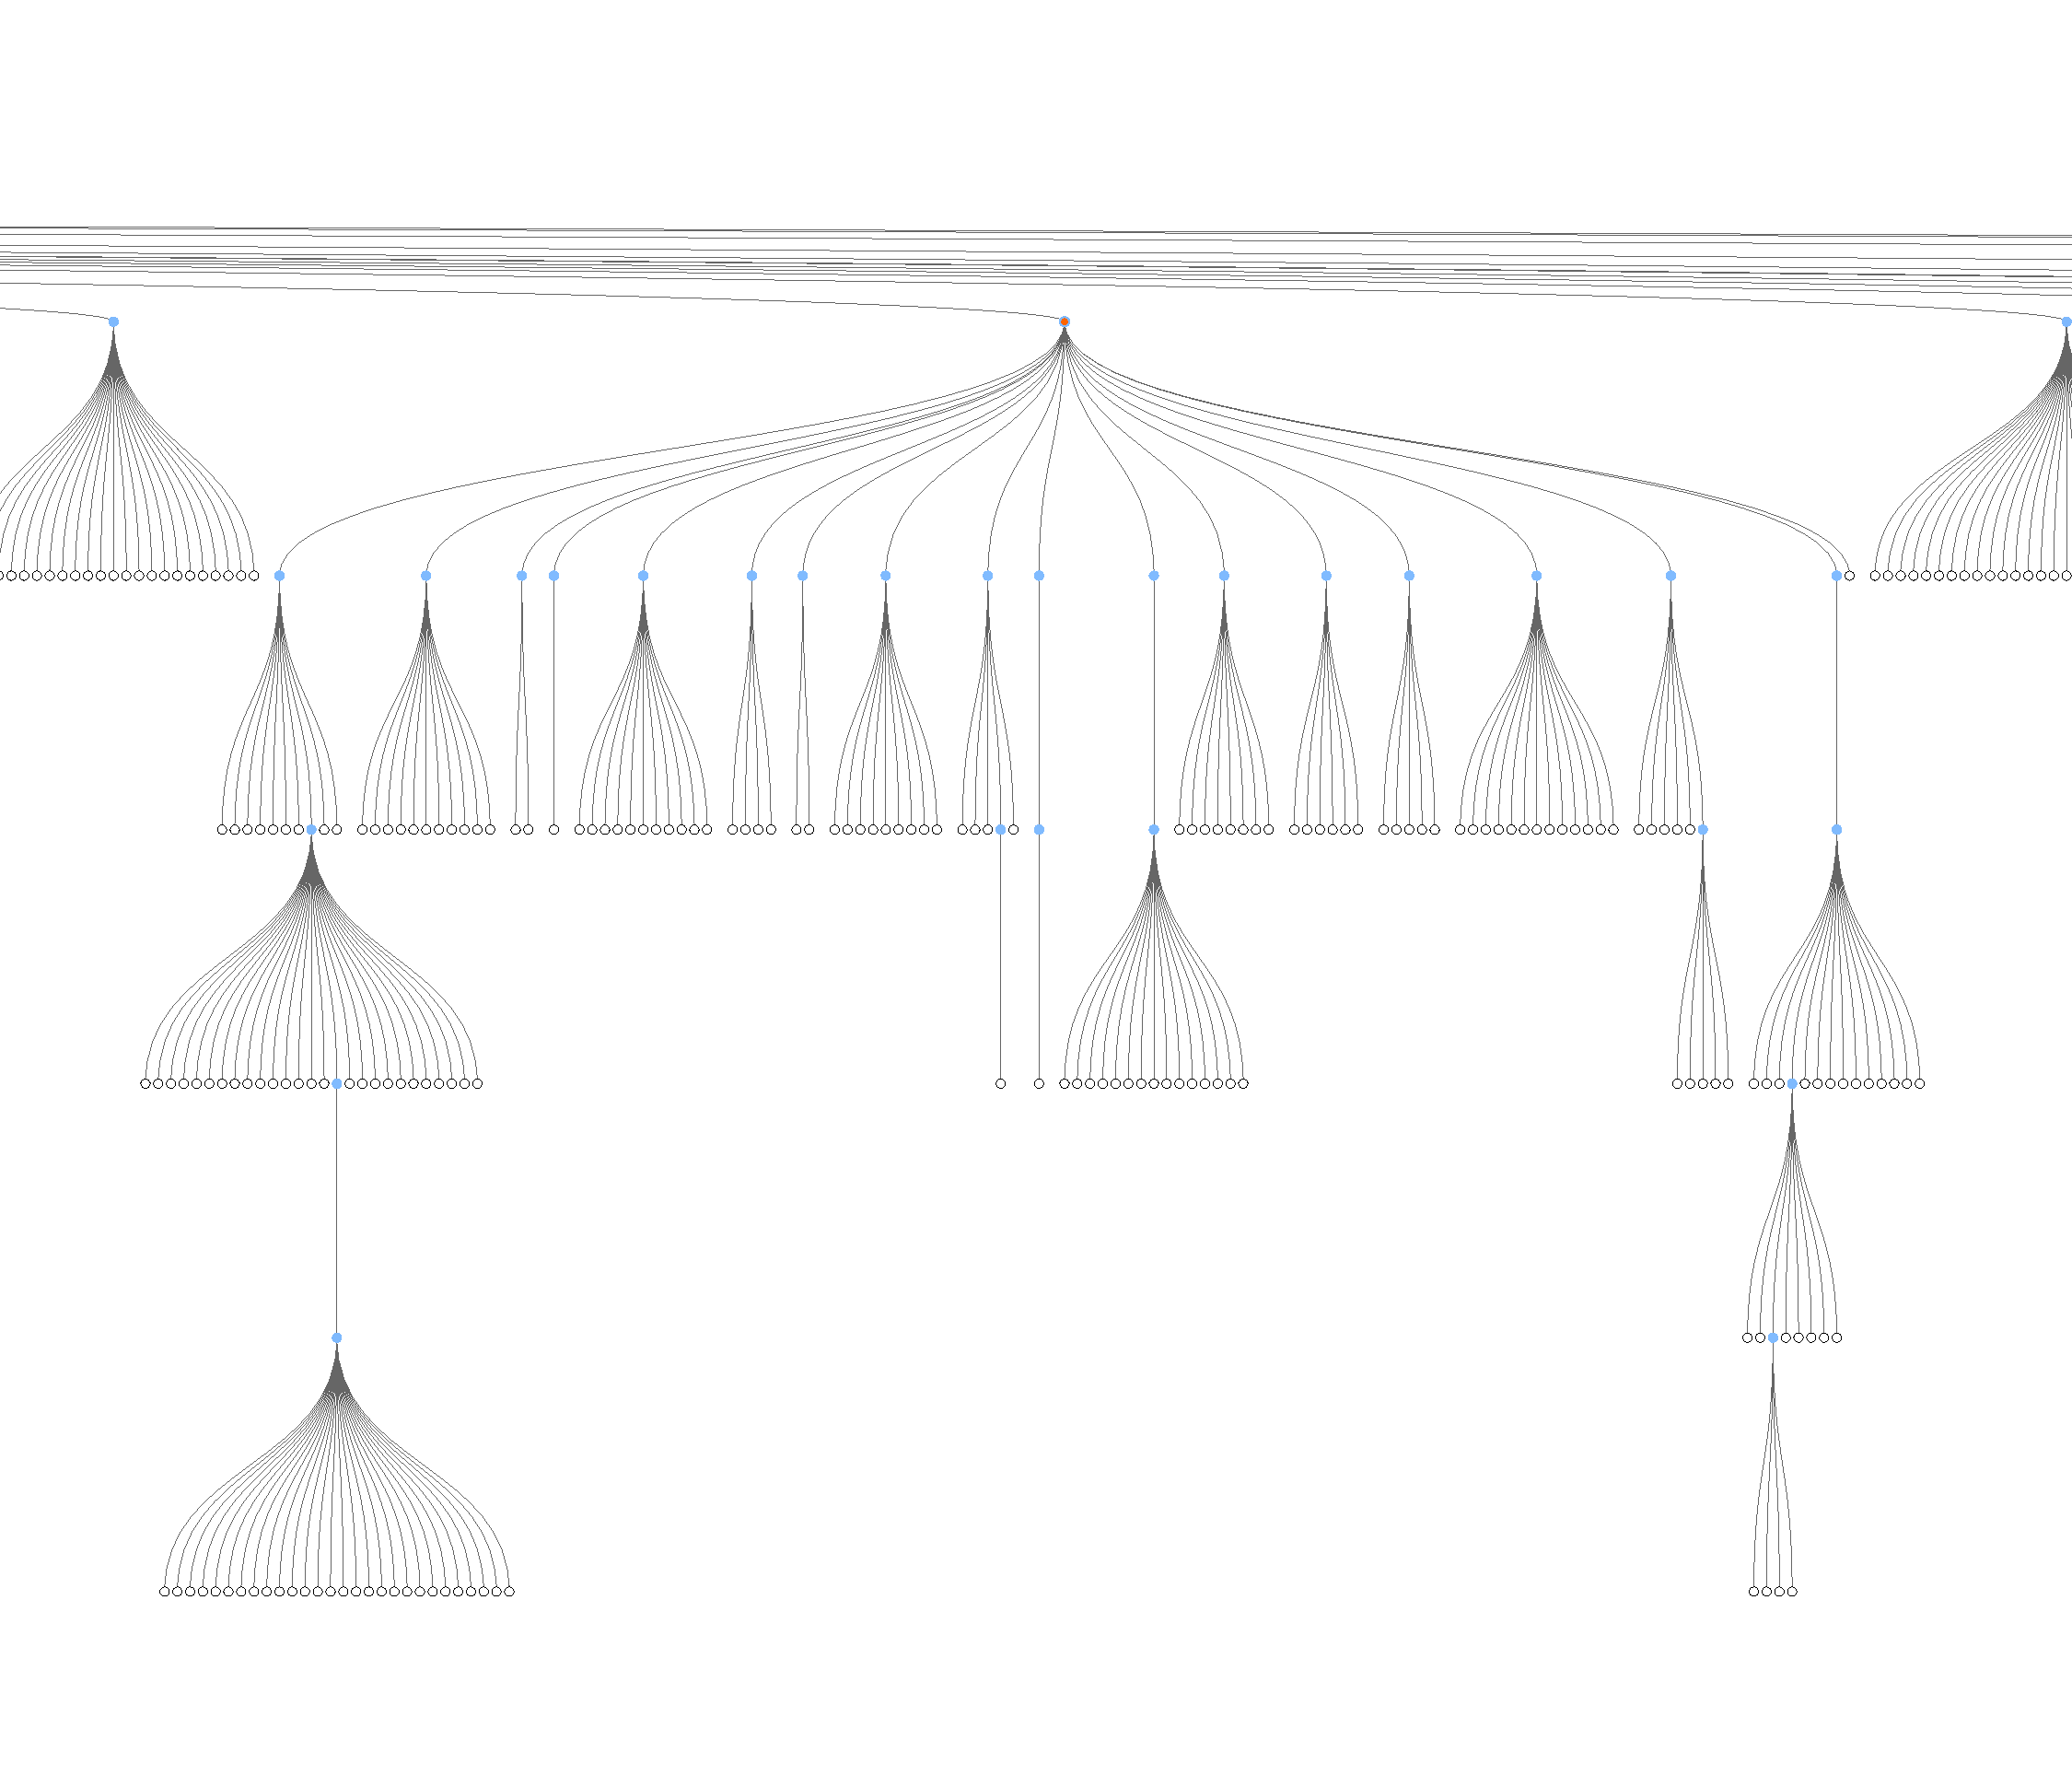
\includegraphics[width=0.47\textwidth]{figures/4dc4_tree.pdf}
        \caption{Merge 4dc4226 is a subtree of 3f17ea6, for the power-management
          module of the kernel}
        \label{fig:reingold_tree}
      \end{figure}

      \begin{figure*}
        \centering
        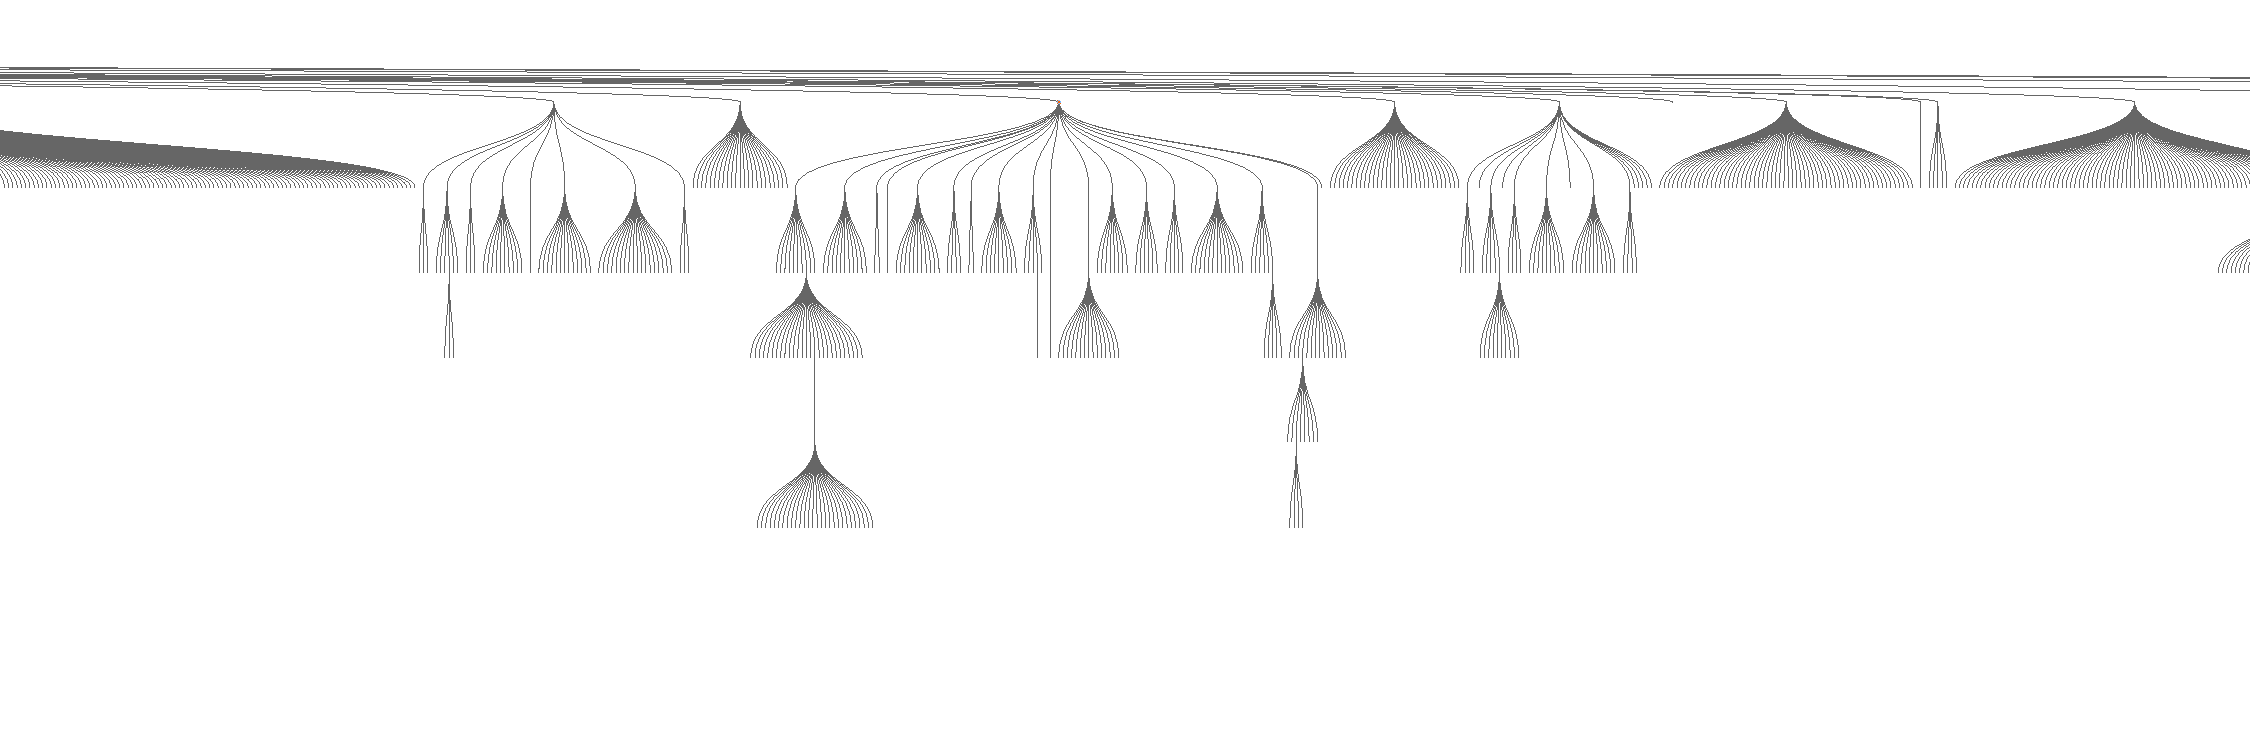
\includegraphics[width=0.98\textwidth]{figures/4dc4_zoom_tree.pdf}
        \caption{Zoomed out view of the Reingold-Tilford tree for merge 4dc4226}
        \label{fig:reingold_tree_zoom}
      \end{figure*}

      The user is initially greeted with their current node centered on
      the screen.  They are able to zoom the tree by scrolling the
      mouse, and clicking and dragging to pan the tree. They can see
      more details about a node by clicking on it, which will provide
      them a link to the specific page for that commit.

\subsubsection{Bubble Tree}

Bubble trees are useful for providing a clear visualization of wide,
hierarchical data\cite{Boardman2000}. The tree structure is represented
by the nesting of nodes; the largest circle is the root, containing all
the other nodes. The smallest circles do not contain any nodes and
therefore represent the leaf nodes.

Our implementation of the bubble tree (Figure~\ref{fig:bubble_tree})
provides the user with a clear picture of where a commit is located in
the merge tree. We highlight the selected commit or merge in red.
Non-selected merges are in a shade of blue determined by the depth of a
node in the tree. The root is the lightest shade of blue, while the
contained merges are progressively darker; the commits are white.

\begin{figure}
        \centering
        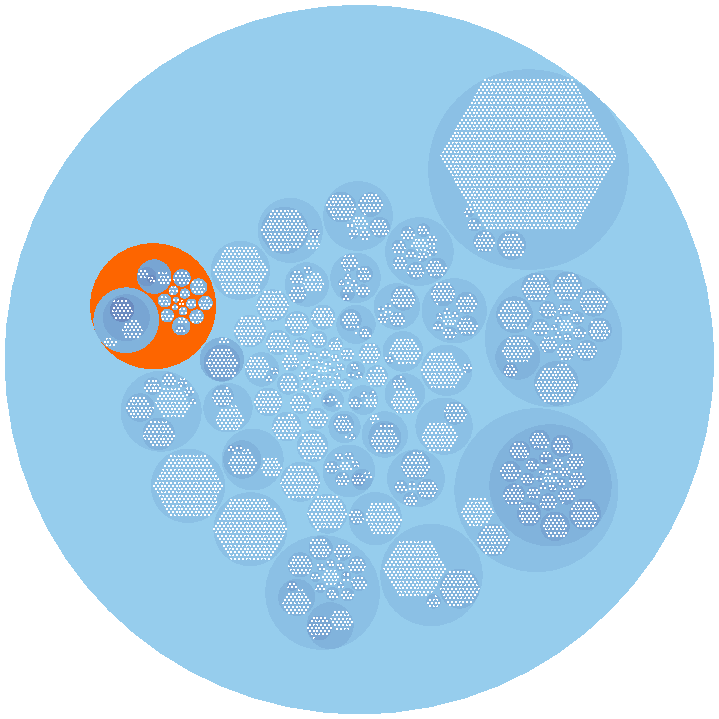
\includegraphics[width=0.47\textwidth]{figures/bubble_tree.pdf}
        \caption{Bubble Tree of merge 3f17ea6, merge 4dc4226 is the currently
          selected merge and is highlighted in orange.}
        \label{fig:bubble_tree}
\end{figure}

The bubble tree doesn't have an implicit way of providing additional
information, placing any text near the nodes makes the tree impossible
to read, so we include a separate pane in the web page. When a user
hovers over a node, the pane shows additional information about the
author and the commit message and a link to the detailed page for that
commit or merge. If the user clicks on a node, the tree will zoom to
that node and the information in the info pane will persist, enabling
the user to click the link. This tree provides an easy mechanism for
users to navigate from the root to the leaves and vice versa.



